\section{Introduction} \label{sec:intro}

% lineeaari tv -> videonauhuri -> on demand -> on demand tv
Watching television used to be a very time-sensitive activity. If one wanted to see a TV program they had to watch it when it was broadcasted. Videocassette recorders %, and later set-top-boxes,
brought the freedom to store programs and to choose freely when to watch them. However, recording programs for later viewing has one major inconvenience. Programs are not broadcasted strictly according to the schedule of the Electronic program guide (EPG). Sometimes programs start earlier or end later than what is stated in the EPG.
To ensure that the entire program is recorded, recording must start before the EPG start time and end after the EPG end time. %, with some margin.
This usually results in some non-program content being included in the recording. Skipping over the non-program content can be frustrating for the person watching the recording.

Knowing when the program truly starts and ends would solve the issue, but this information is not generally available. % commonly transmitted in the broadcast. 
This leaves the option to detect the start and end of the program from the recording. Various artificial intelligence solutions have been devised \cite{berraniNonsupervisedApproachRepeated2008} \cite{ibrahimTVStreamStructuring2011} \cite{kompatsiarisTVContentAnalysis2012} \cite{mansonAutomaticTVBroadcast2010}, but as program content can be quite varied it is difficult to find an universal solution. 
%TODO: check that cited papers are decent

% When video recorders became affordable, they enabled people to record TV programs and watch them whenever. Currently, user-recorded TV programs no longer need to be stored on the users local devices, as content providers are increasingly offering storage space on their own servers for users. 

% NVPR = videonauhuri pilvessä, jonka katsoja jakaa muiden kanssa
Network personal video recorder (NPVR) is a type of service for recording broadcast TV programs for later viewing. Instead of storing recordings on the users local device, NPVR stores recordings on the content providers server. For every program listed in the EPG, a single recording is created and stored on the server. The users who record the same program will receive the same video from the server.

% NPVR ongelma
The start and end times of NPVR recordings are determined by the scheduling information given in the EPG, but some margin is added on both ends to ensure that the entire program is recorded. Similar to storing the recordings locally, this typically leads to non-program content being included in recordings. However, NPVR has a certain advantage over local storage. Users who have recorded the same program will watch the exact same recording, and statistics of which parts of the recording users watch and which parts they skip can be collected and analysed.

The goal of this thesis is to study whether user viewing behaviour can be used to determine when the start and end credits and advertisement breaks occur in an NPVR recording.
%user viewing behaviour can be collected. %As mentioned earlier, this usually result in surplus content being included in the recording. 
%However, it is common that programs are not broadcasted exactly according to the EPG schedule. To ensure that the whole program is recorded, some margin is typically added on both ends of the recording. Thus, NPVR recordings tend to have some non-program content at the beginning and end, in which the users are not interested in. %This extra content is generally uninteresting to the users.
%Furthermore, some programs have also advertisement breaks, which the users typically also want to avoid watching.
%The goal of this thesis is to study whether user viewing behaviour can be used to determine where the start and end credits begin in an NPVR recording.
% motivaatio
I am writing this thesis for an NPVR service provider company. From the perspective of an NPVR service provider, detecting the location of core program content is useful for the following reasons. Firstly, less storage space is needed if the surplus contet is discarded. Secondly, it is convenient for the customers if the relevant content of a recording is pre-identified and they do not have to search for it.
%Secondly, when the customers want to watch multiple episodes of a series in a row, it is convenient for them if a link to the next episode is displayed during the closing credits.

% rajaus
% User viewing behaviour might also be useful for detecting starting credits and advertisement breaks, but on this thesis I will focus on the closing credits detection to narrow down the topic. I will also restrict the examined recordings to TV series with multiple episodes and at least one hundred views per episode.

% sisältö ja rakenne
%The main goal of this thesis is to study whether user viewing behaviour can be used to detect start and end credits and advertisement breaks of NPVR recordings.
%TODO: refs
The thesis is structured as follows. Section \ref{sec:data} gives an overview on the characteristics of the viewing behavioiur data. Section 3.1 discusses the theoretical background of signal change point detection from the perspective of this specific use case. Result evaluation and validation is discussed in section 3.2. In section 4.1 the Python scientific library \texttt{ruptures} is used to detect change points. The results are evaluated in section 4.2. Section 5 discussion considers the viability of using user viewing behaviour for change point detection, based on the previous sections. Lastly, the main points of this thesis are summarised in section 6 conclusions.

\section{User viewing behaviour data} \label{sec:data} % or use case, signal type, data properties etc.

%\subsection{Structure of the data} \label{subsec:data}
% what is the user viewing behaviour data 
Whenever an NVPR video is watched by a user, certain metrics about the viewing event are saved. %metrics are collected from the viewing event. %This is done in order to monitor the amount of views and the user experience quality. 
The main reason for collecting viewing metrics is the monitoring of the amount of views and the user experience quality. From the metrics of one view, it can be calculated which parts of the video the user watched and which parts they skipped. When this data is aggregated from multiple views of the same recording, an overview of what parts of the recording users typically watch is acquired. This type of recording specific aggregated view count is referred to as user behaviour data in this thesis. %examined in this thesis.
%The change point detection will be done based on this data.

% core program content vs other stuff
The content of an NPVR recoring %consists of
can be categorised into start credits, core program content, advertisement breaks, end credits and non-program content at the very beginning and end of a recording. Every recording has core program content and end credits, but not all recordings have start credits or advertisement breaks. Core program content is considered relevant for the users, while non-program content and advertisement breaks are considered irrelevant. The relevancy of start and end credits is something in between, since many users prefer to skip them, but they still belong to the program and are not extra content as such.

% change points definition
%For the purpose of
In this thesis, starting credits, advertisement breaks and end credits will be referred to as change segments. The start and end points of the aforementioned will be referred to as change points. The goal of this thesis is to find a suitable method to determine at least the approximate location of change points.% and preferably even the start and end timestamps of change points with some small margin of error. % 1 vs 2 change points per event

\begin{figure}[h]
    \centering
    \begin{subfigure}[b]{\textwidth}
       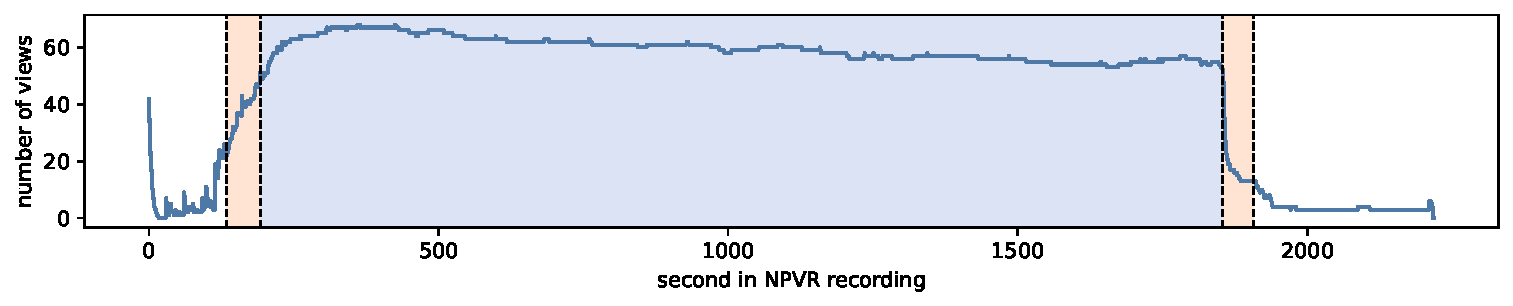
\includegraphics[width=1\textwidth]{../plots/sitcom.pdf}
       \caption{30 min sitcom episode without advertisements, 100 views}
       \label{fig:sitcom_viewing_behaviour} 
    \end{subfigure}
    
    \begin{subfigure}[b]{\textwidth}
       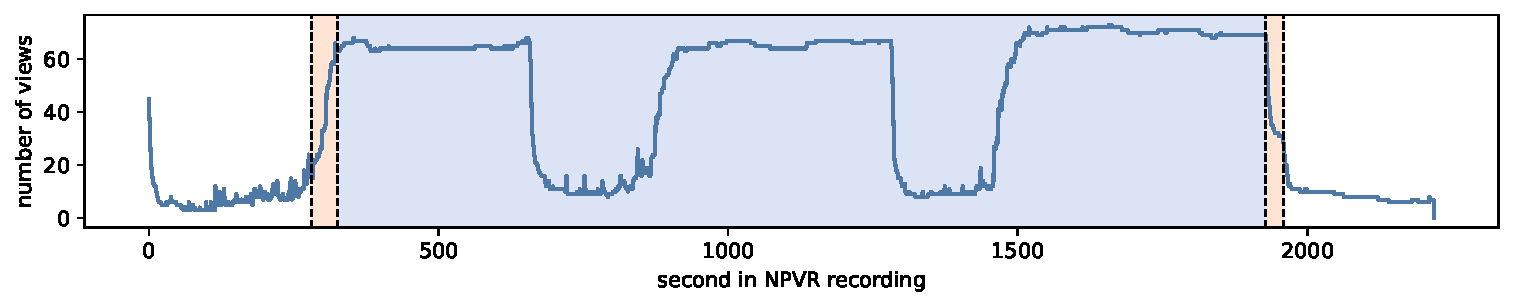
\includegraphics[width=1\textwidth]{../plots/soap_opera.pdf}
       \caption{30 min soap opera episode with two advertisement breaks, 100 views}
       \label{fig:soap_opera_viewing_behaviour}
    \end{subfigure}
    \caption{Visualisation of user viewing behaviour for two example recordings}
    %\caption{Visualisation of user views count for each second in two example NVPR recordings}
    \label{fig:user_viewing_behaviour}
\end{figure}

% example
Two examples of %NVPR recording
user viewing behaviour data are illustrated in Figure \ref{fig:user_viewing_behaviour}.
The data in both figures consists of a sample of 100 user views, but the views are from two different TV programs. Figure \ref{fig:sitcom_viewing_behaviour} views are from a sitcom episode and Figure \ref{fig:soap_opera_viewing_behaviour} views are from an episode of a soap opera. The episodes are divided into one second-long segments, and calculated for each segment is the number of user views in which the segment was watched. The segments are plotted on the horizontal axis, and the number of user views per segment is plotted on the vertical axis. For example, 63 users from the sample of 100 users watched the part of the sitcom episode between 0:10:00 - 0:10:01 (600 on the horisontal axis in Figure ref{fig:sitcom_viewing_behaviour}).

The change segments are indicated with a red background and the change points are marked with a vertical dashed line. In Figure \ref{fig:soap_opera_viewing_behaviour} there are a total of four change segments, which correspond to start credits, two advertisement breaks and end credits, respectively. Figure \ref{fig:sitcom_viewing_behaviour} episode has no advertisement breaks. The change points were checked by hand from both of the videos. It can be seen from the figures that a steep increase in views occurs when the actual program content begins, and correspondingly there is a steep decrease in views when the program content shifts to advertisements or closing credits.
%TODO: subsection about data cleaning
\newpage
\section{Theoretical background} \label{sec:background}

\subsection{Signal change detection} \label{subsec:methods} % for this specific case

%definition
%classification:
%methods (the paper, bayes, something else)
%online/offline
%(un)known nof points 
%cost function, parametric/non-parametric
%search method, optimal/approximate (accuracy vs performance)

%tie to npvr case & definition
Locating video content changes from user viewing behaviour time series data can be formulated as a signal processing problem, more precisely as a change point detection problem. Signal change point detection is quite widely researched topic, since it has applications in multiple fileds such as network traffic data analysis \cite{levy-leducDetectionLocalizationChangepoints2009} \cite{lung-yut-fongDistributedDetectionLocalization2012}, bio-informatics \cite{liuChangepointDetectionMethod2018} \cite{vertFastDetectionMultiple2010} and climatology \cite{reevesReviewComparisonChangepoint2007} \cite{verbesseltDetectingTrendSeasonal2010a}.
% TODO: add examples and check that the papers make sense

% offline
Change point detection problems can be divided into two main categories, depending on whether the change detection must be done for incoming data in near real-time, or not. Methods solving the former case are referred to as online algorithms. Offline algorithms solve the latter case, and they differ from the online algorithms by getting the entire dataset as input and typically being more computationally complex, but also by detecting the changes more accurately.

% unknown number of changes
Offline methods can be divided into two categories, based on whether the number of changes in the dataset is known beforehand, or not. If the number of change points is not known, an extra step is needed to determine it. There are multiple methods for doing this.

%Literature review by Truong et al. \cite{truongSelectiveReviewOffline2020} studied and compared different offline change point detection methods. The publication classified change point detection methods according to how the homogenuity was measured and how the segments where to evaluate the homogenuity were chosen.
%The paper identified three components that are present in all change 
%classified change point detection methods according to three criteria. 
% search methods

% cost functions

% TODO: prioritize theoretical section 
% TODO: check if median is not that good because there aren't that many outliers
% TODO: explain why l2 works better than l1 for this use case, not priority but nice to have
% TODO: figure out how penalty works, important (read pelt)

\begin{equation}
    c_{L_2}(y_{a.b}) = \sum^b_{t=a+1} \left\lVert y_t-\overline{y}_{a.b} \right\rVert ^2_2%\hat{} \sum_{n = 1}^{\infty}  \left\lVert \right\rVert \overline{} 
    \label{eq:l2}
\end{equation}

% constraint functions when k is unknown

\subsection{Result evaluation and validation} \label{subsec:validation}

In order to asses the accuracy of the output of the chosen algorithms, there are some metrics as presented in Truong et al. \cite{truongSelectiveReviewOffline2020} literature review.

%\subsubsection{Change point detection specific methods}

%There are multiple methods for 
%Truong et al. \cite{truongSelectiveReviewOffline2020} literature review introduces the following 
% specific to change point detection:

% Annotation error
% kuinka paljon mallin antamien muutospisteiden määrä eroaa todellisesta määrästä

% Hausdorff
% kuinka suuri on isoin ero mallin antamasta muutoskohdasta lähimpään todelliseen muutoskohtaan

% Rand index
% kuinka suuren osan koko otoksesta malli on luokitellut oikein

% F1-Score
% precision (kuinka suuri osa löydetyistä todellisia), recall (kuinka suuri osa todellisista löydetty)

% general:

\section{Empirical research} \label{sec:casestudy}

\subsection{Ground truth} \label{subsec:groundtruth} %ground truth, sample data

In order to evaluate how well a method detects change points, a ground truth is needed for comparison. Ground truth can be obtained by having a person look at a video recording and having them write down the timestamps of the change points.

I have collected the start and end times of the change points from 174 NPVR recordings by hand with a margin of error of $\pm$ 1 seconds. The sample consists of episodes from 9 different TV series. The recordings are listed in Table \ref{tab:data} categorised by series. The episodes from series 1.-5. were recorded from non-commercial channels, that have no advertisement breaks.
Every recording in the sample has at least one hundred user views.

\begin{table}[h]
    \begin{center}
    \begin{tabular}{|p{15mm}|p{20mm}|p{22mm}|p{28mm}|p{30mm}|} %{|c|c|c|c|c|}
        \hline
        \textbf{\# series} & \textbf{\# episodes} & \textbf{\# ad breaks} & \textbf{episode length} & \textbf{genre}  \\ \hline
        1. & 32 & 0 & 30 min & sitcom\\ \hline
        2. &  8 & 0 & 45 min & drama\\ \hline
        3. & 30 & 0 & 45 min & drama\\ \hline
        4. & 4  & 0 & 50 min & drama\\ \hline
        5. & 10 & 0 & 50 min & drama\\ \hline
        6. & 35 & 1 & 30 min & soap opera\\ \hline
        7. & 31 & 2 & 30 min & soap opera\\ \hline
        8. & 15 & 3 (most) & 60 min (most) & reality show\\ \hline
        9. &  9 & 4 & 90 min & reality show\\ \hline
    \end{tabular}
    \end{center}
    \caption{Sample recordings categorized by series}
    \label{tab:data}
\end{table}

\subsection{Change point detection with \texttt{ruptures} library} \label{subsec:solution}
% cost-function -> probably parametric and pretty simple, pelt accepts only l1, l2 (and rbf)
% search method -> probably optimal (pelt) but approximate methods could be tried
% constraint -> unknown K^* 

% what is ruptures
A Python library called \texttt{ruptures} was used for the change point detection. \texttt{ruptures} is based on the findings of a literature reviw conducted by Truong et al. \cite{truongSelectiveReviewOffline2020} which examined various methods for offline change point detection. Selected algorithms examined in the literature review are implemented in \texttt{ruptures}.

%algos and parameters used
%\texttt{Pelt} (Pruned Exact Linear Time) was used as the search method.

% search method should be optimal 
Choosing the most suitable algorithm %from the library
for this use-case can be done by considering the three aspects of change detection methods discussed in the literature review: cost-function, search method and constraint. Accuracy is more important than low computational complexity, so optimal method is preferable to an approximate one. \texttt{ruptures} has two optimal search methods \texttt{Opt} and \texttt{Pelt}. The difference between them is that \texttt{Opt} works only when the number of change points is know beforehand, and \texttt{Pelt} is used for unknown number of change points. %decides the number of change points accoridng to a linear penalty constraint given by the user.
\texttt{Opt} was first introduced by Bellman \cite{bellmanRoutingProblem1958} for an unrelated problem and \texttt{Pelt} was first indroduced by Killick et al. \cite{killickOptimalDetectionChangepoints2012}. 

% cost function
\texttt{Opt} and \texttt{Pelt} can be used with three different cost functions $c_{L1}$, $c_{L2}$ and $c_{rbf}$. 

%least absolute deviation, least squared deviation (variance), kernel cost function

% output visualisation & comparison to ground truth fig
An example of \texttt{Pelt} output with cost function $c_{L2}$ is visualised in Figure \ref{fig:ruptures_change_detection}. The viewing behaviour data is the same as in Figure \ref{fig:user_viewing_behaviour}. The difference between the figures is that in Figure \ref{fig:ruptures_change_detection} the vertical dashed lines mark the change points determined by \texttt{ruptures} instead of the real changepoints checked by hand. The start and end times of advertisement breaks were found fairly accurately, but for the start and end credits only one change point was found. The change point for the closing credits seems to align with the beginning of the credits. The change point for the start credits falls in the middle of the start credits.


% pruning of data

\begin{figure}[h]
    \centering
    \begin{subfigure}[b]{\textwidth}
       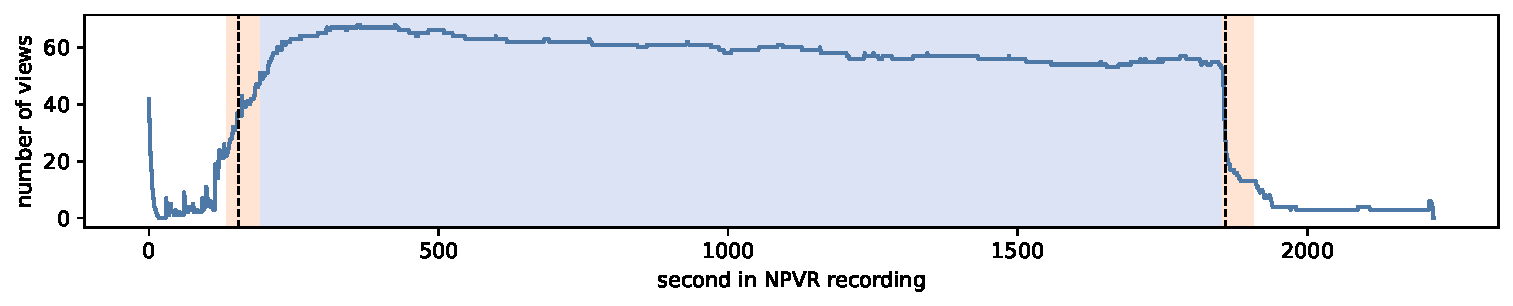
\includegraphics[width=1\textwidth]{../plots/sitcom-pelt_l2_pen30000.pdf}
       \caption{\texttt{Pelt} $c_{L2}$ output for Figure \ref{fig:sitcom_viewing_behaviour} data}
       \label{fig:pelt_sitcom} 
    \end{subfigure}
    
    \begin{subfigure}[b]{\textwidth}
       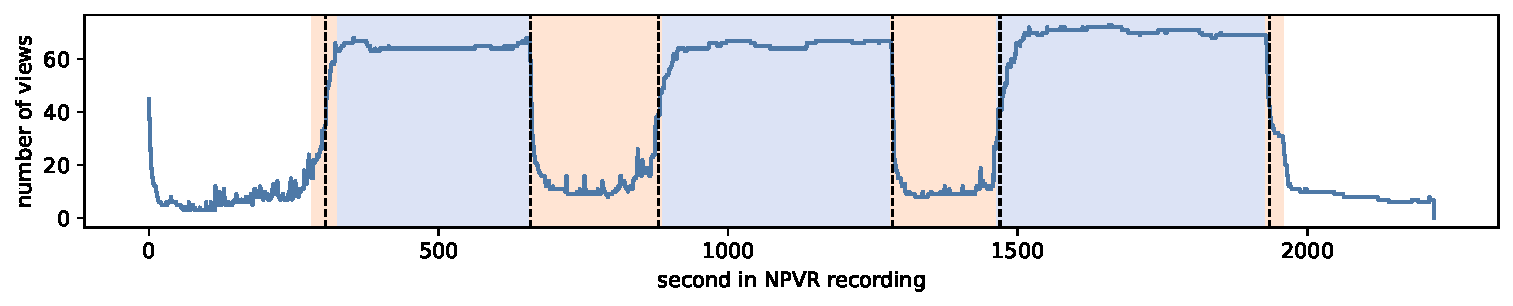
\includegraphics[width=1\textwidth]{../plots/soap_opera-pelt_l2_pen30000.pdf}
       \caption{\texttt{Pelt} $c_{L2}$ output for Figure \ref{fig:soap_opera_viewing_behaviour} data}
       \label{fig:pelt_soap_opera}
    \end{subfigure}
    \caption{\texttt{Pelt} $c_{L2}$ output for Figure \ref{fig:user_viewing_behaviour} data}
    \label{fig:ruptures_change_detection}
    %\caption{Visualisation of user views count for each second in an example NVPR recording}
\end{figure}

%\subsubsection{Opt}

%\subsubsection{Pelt}

\subsection{Results} \label{sec:results}

\section{Discussion} \label{sec:discussion}

% correctly identifying number of changepoints is difficult
It is non-trivial to find an universal solution that works regardless of the number of advertisemet breaks and the length of the recording. When linear constraint is used, like in \texttt{Pelt}, a different penalty value would be optimal for non-commercial and commercial channels.
% separate approach with fixed k = 2 or 4 for non-com channels w no ads
% using multiple models for same data, binary signal processing with ruptures

% is there a difference between different programs or program types?
% how unconventional program structure affects things

% pruning
% data needs to be pruned a bit to get more accurate results
% ways to prune:
% remove views with implausible length (negative or very long)
% remove views which ended before the recording process ended
% maybe remove very short views? (has not been tried out)

% how many views is sufficient for accurate results

% how the amount of views affects the results, and suitable penalty value
% can the start and end times of credits be identified with enough views?

%possible later uses
%detect when whole program is not recorded from k
%train some model to detect changepoints, labeler

\section{Conclusions} \label{sec:conclusions}
